\documentclass{beamer}
\usepackage[utf8]{inputenc}
\usepackage{minted}
\usepackage{prooftree}

\usepackage{tikz} %library per grafi RDF
\usetikzlibrary{positioning, quotes} %per posiziomento relativo dei nodi

\title[Tipi e Ontologie]{Sull'utilità dei sistemi di tipi e dei linguaggi funzionali per la Knowledge Representation}
\subtitle{Stato dell'arte, $\lambda_{DL}$ e possibili direzioni future}
\author[Bafunno, Rovaretto, Zito]{L.~Bafunno, E.~Rovaretto, A.~Zito}
\institute[UniTo]{Dipartimento di Informatica\\
Università degli Studi di Torino}
\date{July 14, 2023}

\newcommand{\singlenodegraph}[1]{
  \tikz{\node [rounded corners, scale=0.9, draw, fill=gray!30, font=\footnotesize] {#1}}
}
\usetheme{Boadilla}
\usecolortheme{default}
\AtBeginSection[]
{
	\begin{frame}
		\frametitle{Contenuti}
		\tableofcontents[currentsection, hideothersubsections]
	\end{frame}
}
\begin{document}
	\maketitle
	\begin{frame}
		\frametitle{Contenuti}
		\tableofcontents[hideallsubsections]
	\end{frame}
	\section{Motivazioni della tesi}
\begin{frame}
	content
\end{frame}
	\chapter[Concetti preliminari]{Concetti preliminari}\label{chap:preliminaries}
Per poter considerare l'utilizzo dei tipi per il Web Semantico, è necessario analizzare lo stato dell'arte in cui si ritrova questo ambito di ricerca.
Questo capitolo si presta utile per apprendere il vocabolario utilizzato durante tutta la tesi, nonché fornire approfondimenti su nozioni che potrebbero essere date per scontate.
Verranno riassunte le basi dei linguaggi funzionali, così come le componenti del Web Semantico.
\section[Linguaggi funzionali]{Linguaggi funzionali}

\section[Web Semantico]{Web Semantico}
Il World Wide Web è diventato una consolidata rete di conoscenza, che però presenta il difetto che queste informazioni sono pensate per la fruizione umana, piuttosto che da parte di una macchina. Infatti il linguaggio di rappresentazione delle centinaia di pagine che visitiamo ogni giorno, l’HTML, descrive l’impaginazione delle informazioni visualizzate all’utente. Senza un indicazione che spiega il significato dei dati presenti, un agente intelligente non può interpretarne il significato. Uno degli obiettivi del Web Semantico, termine che risale all'articolo del 2001 di Tim-Berners Lee \cite{berners2001semantic}, è cambiare questo paradigma human-centered, permettendo agli agenti artificiali di interpretare e processare la conoscenza presente senza alcun tipo di aiuto umano. È necessario descrivere le informazioni attraverso metadati espressivi, strutturandoli arbitrariamente, che ne spieghino la semantica in un modo che una macchina possa comprenderla.\\
Nel corso degli anni, nella letteratura sono state presentate diverse soluzioni: dagli albori di questo ambito, in cui i dati erano rappresentati in maniera strutturata e formale dalle ontologie, si è giunti alla rappresentazione superficiale ma efficiente del paradigma dei Linked (Open) Data. Questa sezione vuole introdurre agli standard di rappresentazione e recupero dei dati citati in questo lavoro.



\subsection[Resource Description Framework]{Resource Description Framework}
Il Resource Description Framework \cite{RDFspecification} (RDF d'ora in poi) è una serie di specifiche create da W3C (World Wide Web Consortium) che includono un modello per descrivere risorse web attraverso delle annotazioni, sotto forma di \textbf{triple}. Esse consistono in:
\[ < \text{soggetto},\ \text{predicato},\ \text{oggetto} > \]
Un insieme di queste triple, chiamato \textbf{grafo RDF}, può essere rappresentato come un grafo diretto etichettato in cui ogni tripla descrive un arco dal nodo soggetto al nodo oggetto.
\begin{figure}[h]
    \begin{minipage}{0.3\linewidth}
        \centering
        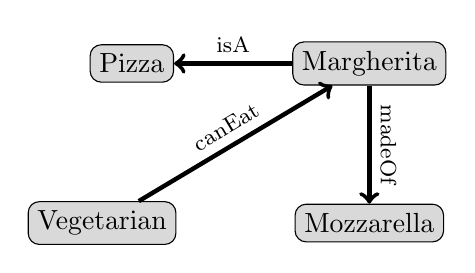
\begin{tikzpicture}[
                node distance = 15mm and 15mm,
                V/.style = {rounded corners, draw, fill=gray!30},
                every edge quotes/.style = {auto, font=\footnotesize, sloped}
            ]
            \begin{scope}[nodes=V]
                \node (1)   {Pizza};
                \node (2) [right=of 1]    {Margherita};
                \node (3) [below =of 2]    {Mozzarella};
                \node (4) [left=of 3]    {Vegetarian};
            \end{scope}
            \draw[->, ultra thick]   (2)  edge["isA"] (1)
            (2)  edge["madeOf"] (3)
            (4)  edge["canEat"] (2);
        \end{tikzpicture}
    \end{minipage}
    \hspace{5mm}
    \begin{minipage}{0.7\linewidth}
        \begin{alignat*}{4}
            G_1 = \{ (\  & \text{Margherita},\  &  & isA,      &  & \text{Pizza}        &  & ),  \\
            (\           & \text{Margherita},\  &  & madeOf,\  &  & \text{Mozzarella}\  &  & ),  \\
            (\           & \text{Vegetarian},\  &  & canEat,\  &  & \text{Mozzarella}\  &  & )\}
        \end{alignat*}
    \end{minipage}
    \caption{un grafo RDF $G_1$ come grafo diretto (sx.) e insieme di triple (dx.)}
    \label{fig:grafoRDF}
\end{figure}

\noindent
Per essere più precisi, \textit{in RDF sia i nodi che i predicati sono risorse}, cioè delle entità nell'universo del discorso d'interesse. A seconda che la risorsa sia una stringa (come Margherita nella \autoref{fig:grafoRDF}) oppure un concetto più astratto è possibile identificarla in due modi diversi: tramite IRI oppure come un letterale. In ogni caso, definire una tripla RDF significa dire che la relazione indicata dal predicato vale fra le risorse indicate dal soggetto e dall'oggetto. Parliamo meglio di questi metodi d'identificazione:
\begin{description}
	\item[IRI (International Resource Identifier)]  Un formato generalizzato di URI che ricorre a un range più ampio di caratteri Unicode, che permette di identificare univocamente una risorsa. È importante sapere che solamente gli IRI vengono utilizzati per identificare i predicati in una tripla, e denotano una \textbf{proprietà}, cioè una risorsa che può essere vista come una relazione binaria.
	Un insieme di IRI destinati all'uso in un grafo RDF è chiamato \textbf{vocabolario RDF} e di solito tutti gli identificatori di uno stesso vocabolario condividono una sotto stringa iniziale comune, che prende il nome di \textbf{namespace}. Per migliorare la leggibilità dei documenti RDF, si utilizza un \textbf{prefisso}, che sostituisce il namespace per abbreviare la lunghezza del identificatore. Ad esempio, per l'IRI \verb|http://example.org/#Margherita| si potrebbe definire il namespace\\ \verb|http://example.org/#| con prefisso \verb|example|; in questo modo la risorsa Margherita può essere identificata con il più corto e leggibile \verb|example:Margherita|. Alcuni esempi concreti possono esseri trovati in \cite{RDFSspecification}.
	\item[Letterali] Rappresentano risorse nel senso di valori numerici, date o stringhe. La codifica di un qualsiasi valore di un letterale è come stringa Unicode, ma è possibile specificare il tipo, identificato da un IRI (e.g. il tipo delle date è \verb|xsd:date|), per permettere di risalire alla vera semantica del valore.
\end{description}
Esiste anche un altro termine che permette di affermare la presenza di un nodo per cui sussiste la relazione, senza nominarlo in maniera esplicita: il \textbf{blank node}. Per fare un paragone, possono essere considerati come variabili esistenziale, in cui il valore non è conosciuto ma si assume che sia presente.

\begin{definition}[Tripla RDF]
	Siano \textbf{I}, \textbf{L} e \textbf{B} rispettivamente gli insiemi infiniti e disgiunti uno a uno delle stringhe IRI, dei letterali e dei blank nodes. Una tripla RDF è una tupla $(s, p, o) \in \textbf{U}\ \cup \textbf{B} \times \textbf{U} \times \textbf{U}\ \cup \textbf{B}\ \cup \textbf{L}.$ in cui s è chiamato soggetto, p il predicato e o l'oggetto.
\end{definition}
\begin{definition}[Grafo RDF]
	Un grafo RDF è un insieme finito di triple RDF.
\end{definition}
\begin{definition}[Grafo RDF]
	Un grafo RDF è un insieme finito di triple RDF.
\end{definition}
IRI (International Resource Identifier),

\subsection{SPARQL CQ}
I grafi RDF vengono interrogati utilizzando le query SPARQL, infatti i grafi vengono memorizzati in database speciali chiamati triplestore, per efficentare le interrogazioni. In questa trattazione utilizziamo un tipo particolare di SPARQL, le query congiuntive, che consistono nella congiunzione di triple pattern, elementi atomici per interrogare un triplestore. \\
\textbf{Abitabilità: } In una query SPARQL, il concetto di abitabilità identifica le query che possono essere abitate da almeno un elemento. Per esempio, se scriviamo una query che richiede tutti i nodi che sono sia di classe Pizza sia di classe Gelato, ovviamente questa query non potrà mai essere abitata, perchè non esistono pizze che allo stesso tempo sono anche dei gelati. Il concetto di abitabilità però non è da confondere con il fatto che essa sia abitata: una query potrebbe essere abitata, ma nel grafo RDF su cui stiamo lavorando non c'è nessun nodo che soddisfa i requisiti. \ 
\begin{figure}[H]
    \centering
    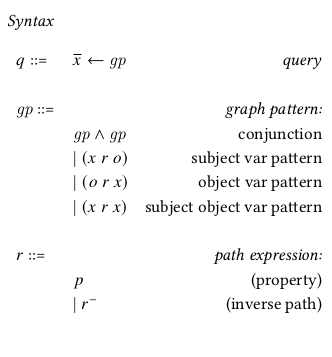
\includegraphics[scale=0.6]{pictures/leinbergSyntax}
    \caption{sintassi delle query \\ SPARQL CQ}
    \label{fig:leinbergerSyntax}
\end{figure}
\newpage
\section[Ontologie]{Ontologie}
La definizione comunemente accettata di ontologia è \textit{una specifica formale ed esplicita di una concettualizzazione condivisa} \cite{goy2015ontologies}. Un modo di rappresentarle è attraverso particolari linguaggi altamente espressivi appartenenti a una famiglia di formalismi chiamati logiche descrittive (DL). Le informazioni sul dominio di interesse vengono espresse in maniera formale tramite formule logiche di due tipologie. Una tipologia fa parte della cosiddetta T-Box e sono asserzioni sulla terminologia, componendo uno schema. L'altra fa parte della A-Box ed è usata per fare asserzioni su individui (astratti), quindi modella le istanze significative. Il T-Box contiene formule logiche (assiomi) che mettono in relazione delle \textit{concept expressions} per modellare il dominio di riferimento, ad esempio il fatto che  uno Student è una Persona. Una \textit{base di conoscenza} è quindi l'insieme di asserzioni presenti sia nel T-Box che nell'A-Box.\\
Nel contesto del Web Semantico, la raccomandazione W3C \textit{Web Ontology Language (OWL)} è una famiglia di linguaggi ontologici altamente espressivi basati sul linguaggio descrittivo $\mathcal{SROIQ}$ \cite{baader2017introductionDL}. Quello che andremo a mostrare noi nella sezione dei costrutti sintattici DL è il più semplice sottoinsieme $\mathcal{ALCOIQ}$.
Grazie alla forma logica delle informazioni, è possibile definire un ragionamento automatico\footnote{\ i.e. tramite un algoritmo deterministico, cioè eseguibile da un computer} che permette di svolgere operazioni di inferenza sugli individui concreti, ad esempio inferire che il nodo \textit{x} di un grafo RDF è uno Studente, ma anche eseguire compiti più astratti, come capire se un concetto è soddisfacibile. Questi compiti sono alla base di ogni reasoner, come ad esempio HermiT \cite{HermiT}, Pellet \cite{Pellet} e Fact++ \cite{Fact++}.\\

\subsection[Logica  descrittiva $\mathcal{ALCOIQ}$]{Logica  descrittiva $\mathcal{ALCOIQ}$}
Questa introduzione e gli esempi sono presi dal libro \cite{baader2017introductionDL}, che contiene un'ottima introduzione alle logiche descrittive. Per non divagare troppo dal motivo per cui spieghiamo questi concetti, ovvero per permettere ai lettori meno esperti delle ontologie di capire la terminologia usata in questa tesi, la logica utilizzata in questa sezione sarà principalmente $\mathcal{ALCOIQ}$. Per questo motivo, useremo anche esempi e tabelle prese dall'introduzione della tesi di dottorato di Leinberger \cite{leinbergerphdthesis}. L'acronimo $\mathcal{ALCOIQ}$ descrive i costrutti sintattici disponibili nel linguaggio (\autoref{fig:SintassiCD}). I costrutti di base sono contenuti in $\mathcal{ALC}$ (\textit{Attributive Language with Complements}), e le estensioni introdotte sono spiegate nella \autoref{tab:ALCOIQExtensions}. \\\\
I linguaggi appartenenti alle logiche descrittive separano le informazioni di un argomento in una parte terminologica (\textit{T-Box}) e una di asserzioni (\textit{A-Box})\footnote{ Nelle estensioni $\mathcal{R}$ del linguaggio $\mathcal{ALC}$, come ad esempio in OWL ($\mathcal{SROIQ}$), esiste una terzo insieme di asserzioni chiamati R-Box. Dentro vengono contenute asserzioni per creare legami fra i ruoli (come equivalenza o sotto-ruolo). Per saperne di più consultare \cite{baader2017introductionDL}}. In altre parole, il T-Box definisce informazioni sulla correlazioni dei concetti (e.g. Studente è una Persona che frequenta un corso), simile a uno schema di un database. L’A-Box descrive invece la rappresentazione concreta dei concetti (e.g. Alice è una Persona), molto più simile alle istanze di una tabella relazionale. La combinazione di entrambe viene definita una \textit{Knowledge Base} (KB).
Nelle logiche descrittive si assume di voler descrivere un’astrazione della realtà d’interesse, e che questa sia popolata da elementi. Per descrivere quest'ultimi utilizziamo tre componenti:
\begin{description}
	\item[Concept expression] Anche chiamato concept description, è un insieme di elementi e può essere visto come un predicato unario. Le concept expressions sono definite a partire dai \textit{nomi di concetti} e dai \textit{nomi di ruolo}. Sono definiti induttivamente dall’insieme di tutte le regole sintattiche del linguaggio considerato (vedi \autoref{fig:SintassiCD}). L’insieme che una concept description rappresenta è chiamato la sua \textit{estensione}. Per esempio, Persona è un concetto, e Alice è un elemento (nell’estensione) di Persona.
	\item[Role expression] relazione binaria sugli elementi. È definito atomicamente da un \textit{nome}. L'unico altro costrutto in $\mathcal{ALCOIQ}$ è il ruolo inverso, che non è nient'altro che la coppia di entità in ordine inverso. Se un ruolo \textit{r} mette in relazione un elemento con un altro, si definisce quest’ultimo un \textit{r}-filler del primo (es. Alice \textit{insegna} C, C è un \textit{insegna}-filler di Alice).
	\item[Linguaggio concettuale] il linguaggio formale al centro di uno specifica logica descrittiva. Permette di costruire concept expressions e role descriptions partendo da nomi di concetti, nomi di ruoli e altre primitive.
\end{description}

Di solito un linguaggio DL permette di costruire concetti utilizzando gli operatori comuni alla logica del prim’ordine (e.g. $\sqcap, \sqcup, \exists, \forall \text{ e } \neg)$, ma ci possono essere varie estensioni che possono essere considerate per un linguaggio. L'estensione che può risultare più strana nella \autoref{fig:SintassiCD} è la regola (Restrizione num. richiesto), che richiede che permette di esprimere il vincolo di avere almeno \textit{n} \textit{r}-filler della concept expression C. Per fare un esempio servirebbe definire l'ambito in cui vengono utilizzate le concept e le role expression, che è proprio quello che introdurremo nella sezione successiva.\\
\begin{figure}[b!]
	\begin{center}	
		\begin{minipage}{0.6\textwidth}
			\setlength{\grammarindent}{3em} % increase separation between LHS/RHS 
			\begin{grammar}
				\let\syntleft\relax
				\let\syntright\relax
				<$\mathbf{C}$> ::= $c$ \hfill (Concetto atomico)
				\alt $\{o\}$ \hfill (Concetto nominale)
				\alt $\top$ \hfill (Top)
				\alt $\bot$ \hfill (Bottom)
				\alt $\neg \mathbf{C} $ \hfill (Negazione)
				\alt $\mathbf{C} \sqcap \mathbf{C}$ \hfill (Congiunzione)
				\alt $\mathbf{C} \sqcup \mathbf{C}$ \hfill (Disgiunzione)
				\alt $\exists\ \mathbf{R}. \mathbf{C}$ \hfill (Esistenziale)
				\alt $\forall\ \mathbf{R}. \mathbf{C}$ \hfill (Universale)
				\alt $\ge n\ \mathbf{R} . \mathbf{C}$ \hfill (Restrizione num. richiesto)
				
				<$\mathbf{R}$> ::= $r$ \hfill (Ruolo atomico)
				\alt $\mathbf{R}^-$ \hfill (Ruolo inverso)
			\end{grammar}
		\end{minipage}
		\caption{sintassi delle \textit{concept expressions} $\mathbf{C}$ e delle \textit{role descriptions} $\mathbf{R}$}
		\label{fig:SintassiCD}
	\end{center}
\end{figure}

\begin{table}
	\centering
	\begin{tabular}{c l c}
		\hline
		Estensione & Descrizione & Costrutto \\
		\hline
		$\mathcal{O}$ & Concetti nominali & $\{o\}$\\
		$\mathcal{I}$ & Ruoli inversi & $ \mathbf{R} ^-$\\
		$\mathcal{Q}$ & Restrizione del numero richiesto & $\ge n\ \mathbf{R} . \mathbf{C} $\\
		
		\hline
	\end{tabular}
	\caption{estensioni dei costrutti sintattici nel DL $\mathcal{ALCOIQ}$}
	\label{tab:ALCOIQExtensions}
\end{table}
In questa introduzione vedremo in particolare il linguaggio concettuale su cui si basa una semplificazione di OWL per permettere ai lettori meno esperti di comprendere il codice presente nel \autoref{chap:Implementazione}.
\noindent
Vedremo a breve il significato della semantica di questi costrutti, ma vale la pena di spendere qualche parola su come andranno a essere utilizzati alcuni di essi. In particolare, esistono diversi costrutti per andare a specificare degli insiemi per tutti quegli elementi che sono in relazione con un certo ruolo a un concetto particolare (parliamo di $\exists r. \mathbf{C}$,  $\forall r. \mathbf{C}$ e $\ge n\ \mathbf{R} . \mathbf{C}$). Questo ci permetterà principalmente nel T-Box di dichiarare qualche genere di concetto che deve essere in relazione con qualcosa. Ad esempio, un Celibe è un uomo che non ha consorte, ed è proprio la mancanza a caratterizzare gli elementi nell'estensione di Celibe. Questo si potrebbe andare a caratterizzare con la concept expression $\text{Uomo}\sqcap \neg\ \exists\ \textit{spostatoCon}. \text{Consorte}$.\\
Una cosa da notare è che la regola (Esistenziale) potrebbe essere espressa attraverso la (Restrizione num. richiesto). Infatti, $\exists r. \mathbf{C}$ è intuitivamente equivalente al caso particolare $\ge 1\ \mathbf{R}. \mathbf{C}$. Per un elenco di regole derivate consultare la sezione 2.2.3 di \cite{leinbergerphdthesis}.


\subsubsection*{Semantica DL}
La semantica nelle logiche descrittive è intesa attraverso un'interpretazione $\mathcal{I}$, definita come segue.
\begin{definition}
	Un'interpretazione $\mathcal{I}$ è una struttura del tipo $\mathcal{I} = (\triangle^\mathcal{I}, \cdot^\mathcal{I})$, dove $\triangle^\mathcal{I}$ è un insieme non vuoto chiamato \textit{dominio d’interpretazione} e $\cdot^\mathcal{I}$ è la \textit{funzione di interpretazione} che mappa ogni costrutto alla sua semantica definita nella \autoref{tab:SintaxSemanticsALCOIQ}.
\end{definition}
\noindent
Come è possibile intuire dalla \autoref{tab:SintaxSemanticsALCOIQ}, ai costrutti della logica descrittiva (concetti e ruoli) vengono assegnati dei significati insiemistici.
\begin{table}[t!]
	\centering
	\footnotesize
	\begin{tabular}{ l l l }
		\hline
		\textbf{Costrutto} & \textbf{Sintassi} & \textbf{Semantica}\\ 
		\hline\\
		Concetto atomico & $c$ & $c^\mathcal{I} \subseteq \triangle^\mathcal{I}$\\
		Concetto nominale & $\{o\}$ & $\{o^\mathcal{I}\}$\\
		
		Top & $\top$ & $\triangle^\mathcal{I}$ \\
		Bottom & $\bot$ & $\emptyset$ \\
		Negazione & $\neg C$ & $\triangle^\mathcal{I} \setminus C^\mathcal{I} $\\
		Congiunzione & $C \sqcap D $ & $C^\mathcal{I} \cap D^\mathcal{I}$\\
		Disgiunzione & $C \sqcup D $ & $C^\mathcal{I} \cup D^\mathcal{I}$\\
		Esistenziale & $\exists r . C$ & $\{\ d \in \triangle^\mathcal{I}\ |\ \text{esiste}\ e \in \triangle^\mathcal{I}\ \text{t.c.}\ (d, e) \in r^\mathcal{I}\ \text{ed }\ e \in C^\mathcal{I}\ \}$\\
		Universale & $\forall r. C$  & $\{\ d \in \triangle^\mathcal{I}\ |\ \text{per ogni}\ e \in \triangle^\mathcal{I}\ \text{, allora}\ (d, e) \in r^\mathcal{I}\ \text{ed }\ e \in C^\mathcal{I}\ \}$\\
		Restrizione num. richiesto & $\ge n\ r . C$ & $\{\ o\ |\ \lvert\{ o'\ |\ (o, o') \in r^\mathcal{I}\ \text{ e } o^\mathcal{I} \in C^\mathcal{I} \}\rvert\ \ge n\ \}$ \\
		\hline \\
		Ruolo atomico & $r$ & $ r^\mathcal{I} \subseteq \triangle^\mathcal{I} \times \triangle^\mathcal{I}$\\ 
		Ruolo inverso & $r^-$ & $ \{\ (o, o') \mid\ (o', o) \in r^\mathcal{I}\ \}$
		\\
		\hline
	\end{tabular}
	\captionsetup{justification={centerlast}}
	\caption{sintassi e semantica delle concept expressions \textit{C}, \textit{D}  e del ruolo \textit{r} nella logica descrittiva $\mathcal{ALCOIQ}$ }
	\label{tab:SintaxSemanticsALCOIQ}
\end{table}
\subsubsection*{Knowledge Base $\mathcal{ALCOIQ}$}
Informalmente, possiamo dire che una Knowledge Base $\mathcal{ALC}$ è composta da 2 componenti: T-Box e A-Box. Iniziamo a definire sintassi e semantica delle T-Box.
\begin{definition}
	Dati $C$ e $D$ concept expressions, una General Concept Inclusion (GCI) è un espressione della forma $C \sqsubseteq D$. Un'insieme finito di GCI è detto T-Box. È possibile definire anche $C \equiv D$ come abbreviazione di $C \sqsubseteq D$ e $D \sqsubseteq C$.\\
	Un'interpretazione $\mathcal{I}$ \textit{soddisfa} $C \sqsubseteq D$ (scritto $\mathcal{I} \models C \sqsubseteq D $) se $C^\mathcal{I} \subseteq D^\mathcal{I}$. Un'interpretazione che soddisfa ogni GCI presente in una T-Box $\mathcal{T}$ è chiamata modello di $\mathcal{T}$ (scritto $\mathcal{I} \models \mathcal{T}$).
\end{definition}
\noindent
Una \textit{T-Box} è quindi una rappresentazione della struttura terminologica di un’ontologia. Una \textit{T-Box} contiene tutte le \textit{condizioni necessarie e sufficienti} per un elemento di far parte dell'estensione di un concetto. In questo modo esprime una gerarchia fra concept expressions. Facciamo un esempio per chiarire
\begin{align}
	\tag{$\mathcal{T}_1$.1} \label{eq:T1.1}
	\mathcal{T}_1 = \{&Person \sqsubseteq \exists\ \textit{hasName}.\top,\\
	\tag{$\mathcal{T}_1$.2} \label{eq:T1.2}
	&Student \sqsubseteq \textit{Person}\ \sqcap \ge 1\ attends.Course\ \}
\end{align}
$\mathcal{T}_1$ è una T-Box semplice, ma basterà per mostrare i casi in cui un'interpretazione non è un suo modello. Ad esempio, con riferimento a \eqref{eq:T1.1}, possiamo affermare che se qualche elemento nell'\textit{estensione} di Person non è in relazione \textit{hasName} con un qualsiasi elemento nel dominio dell'interpretazione, allora quell'interpretazione sicuramente non sarà modello per $\mathcal{T}_1$. Andiamo a vedere ora l'interpretazione $\mathcal{I}_1$, che è una degli infiniti possibili \textit{modelli} di $\mathcal{T}_1$.
\begin{align}
	\tag{$\mathcal{I}_1$} \label{eq:I1}
	\triangle^{\mathcal{I}_1} &= \{\ alice,\ bob,\ c1\ ,\ Roberto,\ bar,\ \textit{foo}\}\\
	\tag{$\mathcal{I}_1$.1} \label{eq:I1.1}
	Person^{\mathcal{I}_1} &= \{\ alice,\ bob\ \}\\
	\tag{$\mathcal{I}_1$.2} \label{eq:I1.2}
	Student^{\mathcal{I}_1} &= \{\ bob\ \} \\
	\tag{$\mathcal{I}_1$.3} \label{eq:I1.3}
	Course^{\mathcal{I}_1} &= \{\ c1,\ alice\ \}\\
	\tag{$\mathcal{I}_1$.4} \label{eq:I1.4}
	attends^{\mathcal{I}_1} &= \{\ (bob, c1)\ \}\\
	\tag{$\mathcal{I}_1$.5} \label{eq:I1.5}
	\textit{hasName}^{\mathcal{I}_1} &= \{\ (alice,\ alice),\ (alice,\ Roberto),\ (bob,\ \textit{foo})\ \}
\end{align}
Ci sono vari particolari da notare in questa interpretazione. Partendo dal dominio d'intepretazione definito in \eqref{eq:I1}, si può notare che l'elemento \textit{bar} non compare in nessuna estensione di un concetto definito da $\mathcal{T}_1$. Questo è assolutamente consentito, e dovrebbe far realizzare che non è possibile conoscere la cardinalità di $\triangle^{\mathcal{I}_1}$. Gli unici elementi che possiamo prevedere far parte del dominio sono quelli che si definiscono nell'A-Box. A differenza di \textit{bar}, \textit{foo} e \textit{Roberto} non compaiono in nessuna estensione, però sono rispettivamente \textit{hasName}-filler di \textit{bob} e \textit{alice} \eqref{eq:I1.5}. La definizione di Person in \eqref{eq:T1.1} richiede che un elemento nella sua estensione abbia almeno un \textit{hasName}-filler del concetto $\top$. Essendo \textit{foo} e \textit{Roberto} nell'estensione di $\top$ (cioè $\triangle^\mathcal{I}$), allora questo è perfettamente legale. Inoltre, sempre riguardo alla definizione \eqref{eq:T1.1}, possiamo notare come:
\begin{enumerate}[(i)]
	\item l'elemento \textit{alice} ha due \textit{hasName}-filler,
	\item uno di questi è se stesso.
\end{enumerate}
La regola (Esistenziale) ha come semantica che deve esistere un elemento \textit{r}-filler che appartiene alla (estensione della) concept expressions specificata (\autoref{tab:SintaxSemanticsALCOIQ}), (i) non crea alcun problema. Inoltre, dato che \textit{alice} è nell'estensione della concept expression $\top$, allora anche (ii) è consentito.\\
L'ultimo particolare su cui si può ragionare è il fatto che \textit{alice} sia contemporaneamente nell'estensione di Course e Person. Effettivamente è contraddittorio che una persona possa essere anche un corso. Questo caso può essere considerato un errore di modellazione del dominio, ma non è un errore dell'interpretazione bensì del T-Box $\mathcal{T}_1$. In effetti non c'è alcuna GCI che vieti ad un elemento di essere contemporaneamente in entrambe le estensioni. Quindi logicamente l'interpretazione sta solo assegnando gli elementi seguendo le regole definite dalla T-Box. Se volessimo evitare questo problema potremmo ridefinire l'asserzione \eqref{eq:T1.1} come:
\[ Person \sqsubseteq \exists\ \textit{hasName}.\top \sqcap \neg Course \]
\\
In generale, una T-Box $\mathcal{T}$ permettono di distinguere le interpretazioni che sono o non sono modelli per $\mathcal{T}$, limitando la nostra attenzione a quelle interpretazioni che modellano la porzione di realtà che si vuole modellare. Più GCI sono presenti in $\mathcal{T}$, meno modelli ha. Per la definizione formale di questa proprietà, consultare \cite{baader2017introductionDL}.
Andiamo ora a definire sintassi e semantica dell'A-Box.
\begin{definition}
	\label{def:ABox}
	Siano $\mathbf{I}$ un insieme di nomi d'individui, disgiunto dai nomi di concetti e quelli di ruolo. Per $a, b \in \mathbf{I}$, C una concept expression e $r$ un nome di ruolo, un'espressione della forma
	\begin{itemize}
		\item $a : C$ è detta un'asserzione concettuale, e
		\item $(a, b) : r$ è detta un'asserzione di ruolo.
	\end{itemize}
	Un insieme finito di asserzioni concettuali e di ruolo è detto A-Box.\\
	Una funzione d'interpretazione $\cdot^\mathcal{I}$ deve mappare ogni nome d'inviduo $a \in \mathbf{I}$ ad un elemento $a^\mathcal{I} \in \triangle^\mathcal{I}$. Un'interpretazione $\mathcal{I}$ soddisfa (scritto $\mathcal{I} \models$):
	\begin{itemize}
		\item $a : C$ se $a^\mathcal{I} \in C^\mathcal{I}$, e
		\item $(a, b) : r$ se $(a^\mathcal{I}, b^\mathcal{I}) \in r^\mathcal{I}$.
	\end{itemize}
	Un'interpretazione che soddisfa ogni asserzione concettuale e asserzione di ruolo in una A-Box $\mathcal{A}$ è detta modello di $\mathcal{A}$ ($\mathcal{I} \models \mathcal{A}$).
\end{definition}
\noindent
Si noti che negli assiomi A-Box, \textit{a} e \textit{b} non sono individui concreti, ed è necessario che sia un’interpretazione a stabilire l'elemento corrispondente da assegnare all'individuo "concettuale". Negli assiomi stiamo solo asserendo che valga una relazione del genere, ma non è detto che sia così o che due individui siano diversi. Facciamo un'esempio concreto:
\begin{align}
	\tag{$\mathcal{A}_1$.1} \label{eq:A1.1}
	\mathcal{A}_1 = \{&\textit{Alice} : \text{Person} \sqcap \text{Student},\\
	\tag{$\mathcal{A}_1$.2} \label{eq:A1.2}
	&\textit{CS600} : \text{Course},\\
	\tag{$\mathcal{A}_1$.3} \label{eq:A1.3}
	&\textit{Ph561} : \text{Course}, \\
	\tag{$\mathcal{A}_1$.4} \label{eq:A1.4}	
	&\textit{Bob} : \text{Student}\\
	\tag{$\mathcal{A}_1$.5} \label{eq:A1.5}
	&(\textit{Bob}, \textit{CS600}) : attends\\
\end{align}
\noindent
Questo A-Box ha due particolarità, riguardanti la definizione dell'individuo \textit{Alice}:
\begin{enumerate}[(i)]
	\item È definito come un'individuo del concetto $\text{Person} \sqcap \text{Student}$
	\item anche se è definito come Student, non è stato esplicitato alcun corso che frequenta, al contrario di \textit{Bob}.
\end{enumerate}
In effetti la concept expression presente nella asserzione concettuale \eqref{eq:A1.1} è ridondante, perchè Student è un sottoinsieme (semanticamente parlando) di Person. Non ha senso definirlo così, ma è comunque un'asserzione concettuale lecita. Concentriamoci invece su (ii): dato che abbiamo specificato \textit{Alice} come Student, vuol dire che deve frequentare almeno un corso, ma non abbiamo detto quale, ovvero non c'è nessuna asserzione di ruolo per della forma $(\textit{Alice}, \_) : attends$. Per la semantica definita nella \autoref{def:ABox}, però, la definizione di \textit{informazioni incomplete} non è assolutamente un problema: sarà compito dell'interpretazione, per essere un modello di $\mathcal{A}_1$, di specificare un qualsiasi elemento che faccia parte dell'estensione di Course. Ad esempio, è proposta una possibile interpretazione $\mathcal{I}_2$ (estesa dalla precedente $\mathcal{I}_1$) per cui $\models_{\mathcal{I}_2} \mathcal{A}_2$:
\begin{align}
	\tag{$\mathcal{I}_2$} \label{eq:I2}
	\triangle^{\mathcal{I}_2} &= \{\ alice,\ bob,\ c1\ ,\ Roberto,\ bar,\ \textit{foo}\}\\
	\tag{$\mathcal{I}_2$.1} \label{eq:I2.1}
	Alice^{\mathcal{I}_2} &= Bob^{\mathcal{I}_2} = bob\\
	\tag{$\mathcal{I}_2$.2} \label{eq:I2.2}
	\textit{CS600}^{\mathcal{I}_2} &= \textit{Ph561}^{\mathcal{I}_2} = c1\\
	\tag{$\mathcal{I}_2$.3} \label{eq:I2.3}
	Person^{\mathcal{I}_2} &= \{\ alice,\ bob\ \}\\
	\tag{$\mathcal{I}_2$.4} \label{eq:I2.4}
	Student^{\mathcal{I}_2} &= \{\ bob, alice\ \} \\
	\tag{$\mathcal{I}_2$.5} \label{eq:I2.5}
	Course^{\mathcal{I}_2} &= \{\ c1, \textit{alice}\ \}\\
	\tag{$\mathcal{I}_2$.6} \label{eq:I2.6}
	attends^{\mathcal{I}_2} &= \{\ (bob, c1), (alice, c1)\ \}\\
	\tag{$\mathcal{I}_2$.7} \label{eq:I2.7}
	\textit{hasName}^{\mathcal{I}_2} &= \{\ (alice,\ alice),\ (alice,\ Roberto),\ (bob,\ \textit{foo})\ \}
\end{align}
Il problema (ii) in questa interpretazione è stato risolto assegnando gli individui \textit{Alice} e \textit{Bob} allo stesso elemento, ovvero \textit{bob}. In effetti, così \textit{Alice} è a tutti gli effetti nell'estensione di Student, soddisfacendo l'asserzione concettuale. In questa interpretazione, anche l'elemento \textit{alice} è nell'estensione Student, ma i due eventi non sono correlati. Volevamo aggiungere un piccolo gioco mentale. Semplicemente, \textit{alice} adesso è nell'estensione di Student perchè la funzione d'interpretazione di $\mathcal{I}_2$ ha mappato ad \textit{attends} un'insieme in cui è presente anche una coppia in cui compare \textit{alice} come primo elemento.
\\
Ora che abbiamo definito entrambi le componenti di una Knowledge Base, possiamo procedere a darne la definizione
\begin{definition}
	Una Knowledge Base $\mathcal{KB}$ è definita dalla coppia $(\mathcal{T}, \mathcal{A})$, dove $\mathcal{T}$ è un T-Box e $\mathcal{A}$ è un A-Box. Un’interpretazione $\mathcal{I}$ è un modello di $\mathcal{KB}$ ($\mathcal{I} \models \mathcal{KB}$) se contemporaneamente $\mathcal{I} \models \mathcal{T}$ e $\mathcal{I} \models \mathcal{A}$.
\end{definition}
\noindent
In altre parole, un modello di una knowledge base è un'interpretazione che soddisfa contemporaneamente tutte le sue asserzioni, terminologiche e sugli individui.  $\mathcal{I}_2$ ad esempio è un modello della knowledge base $(\mathcal{T}_1, \mathcal{A}_1)$, mentre  $\mathcal{I}_1$ non lo è.
\subsection[Problemi di reasoning]{Problemi di reasoning}
Finora, abbiamo definito le componenti di una knowledge base DL e che cosa significhi per un'interpretazione essere un modello di essa. Di seguito illustreremo le definizioni di alcuni problemi di ragionamento che saranno necessari per capire di cosa si sta parlando principalmente nel \autoref{chap:Implementazione}. In particolare questi problemi sono alla base di ogni reasoner, strumenti in grado di eseguire attività di ragionamento. Tipicamente, nel Web Semantico, questi tool vengono basati su RDFS o OWL.
\begin{definition}
	Sia $\mathcal{A} = (\mathcal{T}, \mathcal{A})$ una knowledge base $\mathcal{ALC}$, C e D concept expressions e b un nome d'individuo. Diciamo che:
	\begin{enumerate}[(i)]
		\item C è soddisfacibile rispetto a $\mathcal{T}$, scritto $\mathcal{T} \models C$, se esiste un modello $\mathcal{I}$ di $\mathcal{T}$ e qualche $d \in \triangle^\mathcal{I}$ tale che $d \in C^\mathcal{I}$.
		\item C è sussunto da D rispetto a $\mathcal{T}$, scritto $\mathcal{T} \models C \sqsubseteq D$, se $C^\mathcal{I} = D^\mathcal{I}$ per ogni modello $\mathcal{I}$ di $\mathcal{T}$.
		\item C e D sono equivalenti rispetto a $\mathcal{T}$, scritto $\mathcal{T} \models C \equiv D$, se $C^\mathcal{I} \subseteq D^\mathcal{I}$ per ogni modello $\mathcal{I}$ di $\mathcal{T}$.
		\item $\mathcal{K}$ è consistente se esiste un modello per $\mathcal{K}$
		\item b è un'istanza di C con rispetto a $\mathcal{K}$, scritto $\mathcal{K} \models b : C$ se $b^\mathcal{I} \in C^\mathcal{I}$ per ogni modello $\mathcal{I}$ di $\mathcal{K}$
	\end{enumerate}
\end{definition}
\noindent
Tutte questi problemi possono essere ridotti alla verifica della \textit{consistenza} di una base di dati (Teorema 2.17 \cite{baader2017introductionDL}). Questo significa che è possibile usare un algoritmo per la consistenza per decidere tutti i problemi precedenti. Si noti, tuttavia, che ci sono altri problemi di ragionamento non menzionati la cui riduzione non è possibile, ed anche se lo fosse la complessità del problema sarebbe intrattabile. Uno di questi è decidere le risposte esatte di una conjunctive query, per cui nel linguaggio $\mathcal{SROIQ}$ (proprio quello di OWL) la sua decidibilità è una questione ancora non risolta, mentre per lo stesso linguaggio la verifica della consistenza è decidibile e \textsc{N2ExpTime} completo \cite{baader2017introductionDL}. Non andremo ad approfondire nel dettaglio la complessità, per i lettori interessati su questa questione consigliamo di approfondire il Capitolo 5 e 7 di \cite{baader2017introductionDL}.


	\chapter[Stato dell'arte]{Stato dell'arte}
Per poter considerare l'utilizzo dei tipi per il Web Semantico, è necessario analizzare lo stato dell'arte in cui si ritrova questo ambito di ricerca.
Questo capitolo si presta utile per apprendere il vocabolario utilizzato durante tutta la tesi, nonché fornire approfondimenti su nozioni che potrebbero essere date per scontate.
Verranno riassunte le basi dei linguaggi funzionali, così come le componenti del Web Semantico.
\section[Linguaggi funzionali]{Linguaggi funzionali}
\section[Web Semantico]{Web Semantico}
Il World Wide Web è ormai una gigantesca e consolidata rete di conoscenza, che però nasconde un difetto fondamentale per l'utilizzo di queste informazioni da parte di un agente artificiale. Infatti il linguaggio di rappresentazione, HTML, è stato pensato per la fruizione umana dei suoi contenuti piuttosto che di una macchina. Ciò rende difficile per quest'ultime capire il significato delle informazioni presenti nel web. Uno degli obiettivi del Web Semantico, presentato per la prima volta nel 2001 in \cite{berners2001semantic}, è cambiare questo paradigma human-centered, permettendo agli agenti artificiali di interpretare e processare la conoscenza presente senza alcun tipo di aiuto umano. È necessario descrivere le informazioni attraverso metadati espressivi, strutturandoli arbitrariamente, che ne spieghino la semantica in un modo che una macchina possa comprenderla.

Nel corso degli anni, nella letteratura sono state presentate diverse soluzioni: dagli albori di questo ambito, in cui i dati erano rappresentati in maniera strutturata e formale dalle ontologie, si è giunti alla rappresentazione superficiale ma efficiente del paradigma dei Linked (Open) Data. Questa sezione vuole introdurre agli standard di rappresentazione e recupero dei dati citati in questo lavoro.

\subsection[Resource Description Framework]{Resource Description Framework}
Il Resource Description Framework\footnote{https://www.w3.org/RDF/} (RDF d'ora in poi) è una specifica W3C (World Wide Web Consortium) che fornisce un modello per descrivere risorse nel Web attraverso delle annotazioni. Un termine (o \emph{tripla}) RDF è della forma:
\[ < \text{soggetto},\ \text{proprietà},\ \text{oggetto} > \]
Un'insieme di triple, chiamato un grafo RDF, permettono di descrivere un grafo diretto etichettato dove le risorse descritte sono i nodi e le proprietà sono gli archi.
\begin{figure}[h]
  \begin{minipage}{0.3\linewidth}
    \centering
    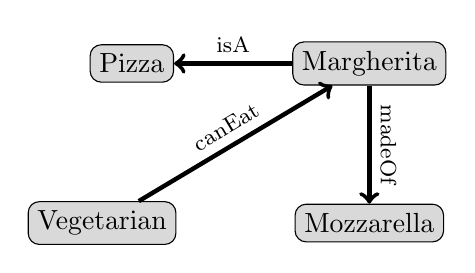
\begin{tikzpicture}[
        node distance = 15mm and 15mm,
        V/.style = {rounded corners, draw, fill=gray!30},
        every edge quotes/.style = {auto, font=\footnotesize, sloped}
      ]
      \begin{scope}[nodes=V]
        \node (1)   {Pizza};
        \node (2) [right=of 1]    {Margherita};
        \node (3) [below =of 2]    {Mozzarella};
        \node (4) [left=of 3]    {Vegetarian};
      \end{scope}
      \draw[->, ultra thick]   (2)  edge["isA"] (1)
      (2)  edge["madeOf"] (3)
      (4)  edge["canEat"] (2);
    \end{tikzpicture}
  \end{minipage}
  \hspace{5mm}
  \begin{minipage}{0.7\linewidth}
    \begin{alignat*}{4}
      G_1 = \{ (\  & \text{Margherita},\  &  & isA,      &  & \text{Pizza}        &  & ),  \\
      (\           & \text{Margherita},\  &  & madeOf,\  &  & \text{Mozzarella}\  &  & ),  \\
      (\           & \text{Vegetarian},\  &  & canEat,\  &  & \text{Mozzarella}\  &  & )\}
    \end{alignat*}
  \end{minipage}
  \caption{Esempio di un grafo RDF $G_1$ (sx.) e sotto forma di insieme di triple (dx.)}
\end{figure}

Invece di chiamare un nodo semplicemente \singlenodegraph{Margherita}. I valori di queste classi (in letteratura \emph{letterali}) possono essere riferimenti tramite URI a risorse Web, oppure
        \section{Implementazione $\lambda_{DL}$}
\subsection{Query SPARQL CQ}
\begin{frame}{Query SPARQL CQ}
    \begin{block}{Definizione}
        Una query SPARQL CQ è un sistema di interrogazione per i grafi RDF, in cui le clausole sono in forma congiuntiva
    \end{block}
    \begin{block}{Query abitabile}
        In una query SPARQL, il concetto di abitabilità identifica
le query che possono ritornare almeno un elemento
    \end{block}
    
    \begin{example}
        Query abitabile: \\
        query x $\leftarrow$ x type Pizza
    \end{example}
    \begin{example}
        Query non abitabile: \\
        query x $\leftarrow$ x type Pizza $\land$ x type Gelato
    \end{example}
 
\end{frame}

\subsection{$\lambda_{DL}$}
\begin{frame}[containsverbatim]{$\lambda_{DL}$}
\blue{Martin Leinberger} nella sua tesi di dottorato propone il \blue{$\lambda_{DL}$}, un \blue{$\lambda$-calcolo tipato}
per poter lavorare con ontologie e avere controlli statici sulle interazioni con esse. Le novit\`a principali sono:
\begin{itemize}
\item Liste e operazioni su di esse come head e tail
\begin{example}
\begin{minted}{haskell}
["L", "a", "y", "t", "o"]
\end{minted}
\end{example}
\item Record e la proiezione su una label
\begin{example}
\begin{minted}{haskell}
{y = 10, i = 0}
\end{minted}
\end{example}
\item Query SPARQL CQ
\begin{example}
\begin{minted}{haskell}
query x <- x type Student
\end{minted}
\end{example}
\end{itemize}
\end{frame}

\begin{frame}[containsverbatim]{$\lambda_{DL}$}
    Per dare un \blue{tipo} ai nodi del grafo RDF, ottenuti dall'esecuzione delle Query SPARQL CQ, \`e stato aggiunta ai tipi standard la \blue{Concept Expression}
    della logica descrittiva:
    ~\\
    \begin{example}
        $K_4 = $\{Student $\sqsubseteq$ Person
        \\Professor $\sqsubseteq$ Person\}
        \begin{minted}[escapeinside=||,mathescape=true, autogobble]{ocaml}
            (head (query x <- x type Student)).x : Student 
        \end{minted}
    \end{example}
    ~\\
Siccome \blue{Student~$\sqsubseteq$~Person} l'espressione ha anche tipo \blue{Person}.
\end{frame}

\subsection{Sull'implementazione del $\lambda_{DL}$}
\begin{frame}{Sull'implementazione del $\lambda_{DL}$}
    Questa implementazione del calcolo di Leinberger prende ispirazione dell'implementazione in Scala dell'autore, ma è originale ed è la prima implementazione di $\lambda_{DL}$ che viene fatta in OCaml. 
    \\\`{E} strutturata in due moduli:
    \begin{itemize}
        \item Modulo OCaml: scritto nell'omonimo linguaggio funzionale. 
        \item Modulo Reasoner: scritto in Java.
    \end{itemize}
\end{frame}

\subsection{Sull'implementazione del $\lambda_{DL}$: OCaml Module}
\begin{frame}{Sull'implementazione del $\lambda_{DL}$: OCaml Module}
    Il modulo OCaml si occupa di parsificare la query, inferire gli assiomi e invocare il modulo Reasoner.
    \begin{block}{Tipi di supporto}
        Il modulo si avvale di alcuni Tipi per rappresentare l'informazione in OCaml:
        \begin{itemize}
            \item Il tipo Query, viene usato per rappresentare nel programma le query SPARQL.
            \item Il tipo ClassExpression per rappresentare una concept expression.
            \item Il tipo Axiom, rappresenta un assioma di Leinberger. 
        \end{itemize}
    \end{block}
    \begin{block}{Manchester OWL Syntax}
    Inoltre viene utilizzata come lingua veicolare di dialogo fra il modulo OCaml e il modulo Reasoner.
    \end{block}
\end{frame}

\begin{frame}{Sull'implementazione del $\lambda_{DL}$: OCaml Module}
    % 1 query e tipo query esempio
    % 2 ocaml trasforma query in tipo query 

    \begin{itemize}
        \item Parsifica una query in formato stringa in un tipo Query
        \begin{example}
            query x $\leftarrow$ x type Pizza $\Rightarrow$
            Q (x, SP(V x, TYPE, A Pizza))
        \end{example}
        \item Inferisce gli assiomi di Leinberger sul tipo Query
        \begin{example}
            Q (x, SP(V x, TYPE, A Pizza))
            $\Rightarrow$ 
            (x, Atomic(Pizza))
        \end{example}
        \item Traduce gli assiomi in sintassi di Manchester e li inoltra al Reasoner
        \begin{example}
            (x, Atomic(Pizza))
            $\Rightarrow$ 
            x : Pizza
        \end{example}
    \end{itemize}
\end{frame}

\subsection{Sull'implementazione del $\lambda_{DL}$: Reasoner Module}
\begin{frame}{Sull'implementazione del $\lambda_{DL}$: Soddisfacibilità di un ontologia}
    \begin{block}{Soddisfacibilità di un ontologia}
        Data un ontologia il reasoner HermiT decide se l'ontologia è soddisfacibile, cioè decide se esiste un modello che soddisfa l'ontologia.
     \end{block}
    \begin{example}
        Per esempio, l'ontologia che presenta un unico assioma di sottoclasse tra il concetto atomico X e la congiunzione tra Pizza e Gelato non è soddisfacibile.
    \end{example}
\end{frame}

\begin{frame}{Sull'implementazione del $\lambda_{DL}$: Reasoner Module}
    Il modulo Reasoner si occupa di verificare la soddisfacibilità degli assiomi di Leinberger, avvalendosi del un reasoner HermiT.
    \begin{block}{Comportamento del modulo}
        \begin{itemize}
            \item Il modulo aggiunge gli assiomi di Leinberger ricevuti dal modulo OCaml all'ontologia.
            \item HermiT decide se l'ontolgia è soddisfacibile.
            \item Se lo è vuol dire che la query è abitata, altrimenti no. 
        \end{itemize} 
    \end{block}
\end{frame}
\subsection{Sistema di Tipi del $\lambda_{DL}$}
\begin{frame}[containsverbatim]{Sistema di Tipi del $\lambda_{DL}$}
    Per implementare il sistema di tipi\footnote{\scriptsize Abbiamo preso spunto da "Type and Programming Languages" di Benjamin C. Pierce \\} abbiamo definito i \blue{termini} del linguaggio:
    \begin{block}{data type per i Termini del $\lambda_{DL}$}
    \begin{minted}[escapeinside=&&,mathescape=true, autogobble]{ocaml}
    type Term =
        | TmRecord of info * (string * term) list 
        | TmProj of info * term * string 
        | TmNil of info * ty 
        | TmCons of info * term * term 
        | TmIsNil of info * term 
        | TmHead of info * term 
        | TmTail of info * term  
        | TmQuery of info * var * gp
        | TmRoleProj of info * term * role
        | TmNode of info * string
    \end{minted}
    \end{block}
\end{frame}

\begin{frame}[containsverbatim]{Sistema di Tipi del $\lambda_{DL}$}
Bisogna definire i \blue{tipi} del linguaggio
    \begin{block}{data type per i tipi del $\lambda_{DL}$}
    \begin{minted}[escapeinside=&&,mathescape=true, autogobble]{ocaml}
    type Ty =
          TyTop 
        | TyBool 
        | TyRecord of (string * ty) list 
        | TyArr of ty * ty 
        | TyNat 
        | TyList of ty
        | TyCe of ce
    \end{minted}
    \end{block}
    e definire la funzione che preso un termine restituisce il suo tipo:
    \begin{block}{Funzione typeof}
    \begin{minted}[escapeinside=&&,mathescape=true, autogobble]{ocaml}
    typeof :: Context -> Term -> Ty
    \end{minted}
    \end{block}
\end{frame}

\begin{frame}[containsverbatim]{Sistema di Tipi del $\lambda_{DL}$}
la funzione \code{typeof} \`e implementata seguendo le regole di tipo. Un esempio interessante \`e la regola per dare un tipo alle query:
~\\
\begin{block}{implementazione [T-QUERY]}
\begin{minted}[escapeinside=||,mathescape=true, autogobble]{ocaml}
    let rec typeof ctx t =
        match t with
        |$\vdots $|
        TmQuery(fi, var, gp) ->
            if allSatisfiable(axioms(gp), var) then
            TyList(TyRecord(var, TyCe(Atomic var))) else
                error fi "axioms unsatisibale"
        |$\vdots$|
\end{minted}
\end{block}
\end{frame}

\begin{frame}[containsverbatim]{Sistema di Tipi del $\lambda_{DL}$}
Per il subtyping abbiamo definito la funzione \code{subtype}:
\begin{block}{Funzione subtype}
\begin{minted}{ocaml}
subtype ::  Context -> Ty -> Ty -> Bool
\end{minted}
\end{block}
Ad esempio per il subtyping tra Concept Expression abbiamo:  
\begin{block}{implementazione [S-CONCEPT]}
\begin{minted}[escapeinside=&&,mathescape=true, autogobble]{ocaml}
    let rec subtype ctx tyS tyT =
        tyeqv ctx tyS tyT ||
        match (tyS,tyT) with
        &$\vdots $&
        | (TyCe(ceS1),TyCe(ceT1)) -> subconcept ceS1 ceT1
        &$\vdots$&
\end{minted}
\end{block}
\end{frame}

\begin{frame}{Sistema di Tipi del $\lambda_{DL}$}
    Perch\`e implementare $\lambda_{DL}$?
    \begin{itemize}
        \item Ci ha aiutato a capire meglio come i sistemi di tipi statici possono essere utilizzati con le ontologie.\\~\\
        \item Abbiamo concluso che OCaml \`e un linguaggio adatto per l'implementazione di linguaggi di programmazione e per interfacciarsi con altri linguaggi per fare reasoning su ontologie. \\~\\
        \item \`E stato un ottimo esercizio di programmazione funzionale.\\~\\
        \item Ci ha spinto ad approfondire le ontologie, la logica descrittiva e i linguaggi di programmazione.\\~\\
        \item I risultati ottenuti incoraggiano lo studio su possibili direzioni future sull'utilizzo di linguaggi funzionali e sistemi tipi statici per il Web Semantico.
    \end{itemize}
\end{frame}
	
\chapter[Direzioni di ricerca future]{Direzioni di ricerca future}
\label{chap:FutureWork}

Nei capitoli precedenti abbiamo esplorato una parte dell'esistente lavoro relativo alla ricerca sull'uso dei sistemi di tipi statici nel contesto della 
rappresentazione della conoscenza, in particolare applicati al formalismo delle ontologie OWL \cite{OWL}. In breve, si può pensare di utilizzare i 
linguaggi con sistemi di tipi statici per realizzare modelli e strumenti per  il Web Semantico, come alternative o come supporto statico al reasoning 
dinamico basato sulle logiche descrittive (si vedano l'introduzione nel Capitolo \ref{chap:preliminaries} e una prima survey sullo stato dell'arte nel Capitolo \ref{chap:State-of-art}).

In questo capitolo, proponiamo alcune congetture di direzioni di ricerca future, ispirate da quanto abbiamo imparato dal nostro studio preliminare e dalle 
discussioni con i colleghi esperti di Web Semantico. Al momento, non abbiamo argomenti né formali né empirici per validare queste idee, tuttavia riteniamo 
che siano un punto di partenza promettente per studi successivi.

Ricordiamo che un'ontologia OWL ha due componenti: \textsc{T-Box} e \textsc{A-Box}. I costrutti nella \textsc{T-Box} sono la "componente terminologica" che descrive un dominio di 
interesse, definendone classi e proprietà, similmente a un vocabolario di quel dato dominio. I costrutti di \textsc{A-Box} sono la "componente assertiva", intesi come fatti associati al modello concettuale descritto dalla \textsc{T-Box}. I costrutti \textsc{A-Box} devono essere \textsc{T-Box}-compliant: sono asserzioni che utilizzano il 
vocabolario definito dalla \textsc{T-Box}. I costrutti \textsc{T-Box} sono talvolta associati a classi orientate agli oggetti e i costrutti \textsc{A-Box} associati a istanze di tali 
classi\footnote{Da \url{https://en.wikipedia.org/wiki/Abox}}.

Utilizzare strumenti logici come i sistemi di tipi per fare reasoning potrebbe sembrare una direzione di ricerca che va nel senso contrario 
rispetto alla preferenza corrente dell'applicazione di tecniche sub-logiche, legate soprattutto al machine learning, anche al reasoning nel web 
semantico. Tali tecniche sfruttano talvolta solo dati estratti dalle asserzioni sugli individui (ovvero dai costrutti della \textsc{A-Box}, spesso rappresentati 
come triple RDF e relativo knowledge graph), soprattutto per questioni di efficienza. In effetti, sembra che al presente  la ricerca sulle ontologie abbia 
perso momento, perché nella loro interezza (\textsc{T-Box} e \textsc{A-Box}) sono troppo formalmente complesse per fare ragionamenti totalmente automatizzati (si vedano i 
concetti preliminari nel \autoref{chap:preliminaries}). Tuttavia, ci sembra che ci siano delle potenzialità da esplorare per poter tornare a fare reasoning più 
sofisticato, senza perdere troppo in efficienza.
\\
Ci sono almeno due strade che possiamo percorrere:
\begin{enumerate}
	\item L'utilizzo di linguaggi funzionali tipati, quali Haskell\footnote{\url{www.haskell.org}} e Ocaml\footnote{\url{www.ocaml.org}} per programmare applicazioni che manipolano le ontologie, con il 
	vantaggio di usare linguaggi basati su un alto livello di astrazione, che quindi permettono uno sviluppo del software modulare, più facile da correggere e da 
	mantenere, e anche più vicino al livello simbolico che caratterizza il reasoning semantico. 
	\item Lo studio di sistemi di tipi statici che garantiscano proprietà 
	interessanti ai programmi, certificati dal sistema di tipi stesso. Il fatto di usare tipi statici, cioè controllati a tempo di compilazione (scelta ancora 
	poco adottata nel reasoning semantico, basata sull'uso di interpreti), potrebbe essere una risposta ai problemi di efficienza per certe proprietà che avrebbe 
	senso controllare a priori, e/o nel caso di grandi quantità di dati.
\end{enumerate}

L'esempio principale che abbiamo scelto di mostrare in questo lavoro, il calcolo $\lambda_{DL}$ di Martin Leinberger presentato nella sua tesi di dottorato 
"Type-safe Programming for the Semantic Web" \cite{leinbergerphdthesis} (si veda il \autoref{chap:Implementazione}) è certamente un esempio del \mbox{Punto 2}. Questo calcolo offre un sistema di tipi per decidere a tempo di compilazione se una query SPARQL è abitata, ovvero se è possibile che produca un risultato quando interpretata, oppure al 
contrario, se non abitata, sappiamo già a priori che la query non produrrà alcun risultato.  Il nostro lavoro di implementazione, però, ci ha dato qualche 
indicazione anche relativamente al Punto 1: per esempio, abbiamo scoperto che il linguaggio Ocaml ha delle librerie utili per il parsing e per interfacciarsi 
con la shell del sistema operativo, oltre ad avere un miglior sistema di error management e il vantaggio di non dover usare monadi, come invece avrebbe 
richiesto Haskell.

Concludiamo questo lavoro con una serie di proposte che potrebbero essere esplorate nel futuro, nelle direzioni menzionate sopra. Queste proposte 
nascono da alcuni proficui scambi di idee con Marco Antonio Stranisci, Rossana Damiano e Antonio Lieto del Dipartimento di Informatica dell'Università 
di Torino.

\section{Tipi per il query rewriting}
Il \textit{query rewriting} è una tecnica per mappare una query SPARQL in un'altra \cite{fQuery}, utile nelle situazioni in cui l'utente non ha una conoscenza precisa del vocabolario e 
del lessico utilizzato nell'ontologia di interesse e in cui lo studio approfondito di questa ontologia non sarebbe vantaggioso, normalmente per motivi di tempo. Un esempio semplice potrebbe essere quello di un'ontologia che descrive razze di cani-poliziotto senza avere il concetto \texttt{Cane} esplicito nel suo vocabolario.
Se l'utente utilizzasse \texttt{Cane} nelle sue query, per esempio per cercare tutti i cani con il manto di un certo colore, non otterrebbe nessun risultato. Una combinazione di strumenti per l'analisi del linguaggio naturale e un sistema di tipi che controlli la correttezza (per esempio nel senso di Leinberger \cite{leinbergerphdthesis}) della query trasformata  dopo l'analisi potrebbe essere un buon strumento per il query rewriting. Un'altra applicazione di simili tecniche potrebbe agevolare l'uso di ontologie il cui vocabolario è in una lingua straniera.

Una direzione pratica per fare esperimenti potrebbe essere utilizzare reti di parole implementate sotto forma di dizionari enciclopedici 
basati sulle ontologie come Babelnet \footnote{Si veda \url{https://babelnet.org/}} per misurare una "distanza semantica"  che intercorre fra due lemmi, per poter decidere quale si avvicina di più a quello usato dall'utente. Possiamo immaginare che si misuri la distanza semantica che intercorre fra la parola della query e le parole nel vocabolario dell'ontologia. Quella con la distanza minore sarà la parola riscritta all'interno della query. Ci potrebbero essere ambiguità, intesa come due o più parole semanticamente alla stessa distanza da quella presente nella query. Per ognuna di queste parole semanticamente simili, si genererebbe dunque una query.
Per controllare l'abitabilità delle query riscritte, sapendo che ogni query ha uno e un solo insieme di assiomi alla Leinberger (si veda \autoref{chap:Implementazione}), si potrebbe generare un tipo che è un insieme di assiomi alla Leinberger se la riscrittura è senza ambiguità, oppure un insieme di insiemi di questi assiomi se la query è effettivamente ambigua.

Questa direzione di ricerca potrebbe beneficiare dallo studio degli approcci per la generazione di query SPARQL partendo da query in linguaggio naturale (questi approcci vengono definiti \textit{Text2SPARQL}). Anche se la quantità di letteratura su questi approcci è ancora scarsa, i lavori \cite{Hu2021NaturalLQ, Evseev2020SPARQLQG} e il tool OSCAR \cite{OSCAR} possono fornire un'idea della struttura dei modelli utilizzati.

\section{Tipi per costruire e ristrutturare ontologie}
Nei processi di creazione di un'ontologia, la tendenza attuale è di sfruttare il più possibile risorse esistenti, sfruttando conoscenze organizzate in 
Terminology Services \cite{ledl2016describing,vandenbussche2017linked} o utilizzando \emph{search engine appositi} come 
Swoogle \cite{swoogle} o Watson \cite{watson} per trovare ontologie. I risultati della ricerca vengono poi sottoposti a processi di valutazione 
(\emph{assesment}), comparazione (\emph{comparison}) e integrazione (\emph{integration}) per ottenere i migliori risultati rispetto al dominio d'interesse. Tali attività possono però essere soggette a errori, poiché le ambiguità, le incoerenze e l'eterogeneità delle ontologie esistenti 
possono influire sui risultati rispetto a diversi punti di vista. Si possono avere, infatti, eterogeneità sintattica, terminologica, concettuale e semiotica \cite{carriero2020OntoReuse}. Questo processo di costruzione di un'ontologia è quindi dispendioso a livello di tempo perché richiede un'accurata verifica da parte degli esperti di ontologie, di cui non è possibile rimuovere il contributo dal processo creativo. L'obiettivo di questa direzione di ricerca sarebbe fornire allo sviluppatore degli strumenti formali da utilizzare durante il processo di creazione/evoluzione di un'ontologia, per aiutarlo nel capire se il suo processo stia effettivamente producendo il risultato desiderato (per esempio offrendo una nozione precisa di equivalenza tra ontologie) e/o suggerire cambiamenti o entità da riutilizzare o aggiungere, sfruttando proprietà come la composizionalità (ovvero la proprietà che garantisce la correttezza della composizione delle parti di un artefatto sviluppate separatamente, posto che le parti obbediscano a certe condizioni), tipica dei linguaggi tipati staticamente. Vista la tendenza attuale di sviluppare un'ontologia partendo da risorse ontologiche esistenti, la proprietà di composizionalità applicata alle ontologie potrebbe automatizzare parte dei compiti di ristrutturazione delle risorse ontologiche da riutilizzare, come la modularizzazione, per considerare solo la parte rilevante per il processo in atto. Un punto di partenza promettente è la metodologia NeOn \cite{NeOn}, che offre una serie di scenari che sono di supporto ai processi di creazione e evoluzione delle ontologie. Uno di questi scenari propone una lista di criteri comparativi per valutare la bontà delle soluzioni possibili (si veda il \autoref{chap:State-of-art}).

Per questa direzione di ricerca servirebbe un caso di studio che potrebbe beneficiare di tali strumenti formali, utili nel caso in cui si voglia progettare 
da zero una nuova ontologia o nel caso di "major changes" di ontologie già esistenti. Al presente sono disponibili ontologie molto generali, ben stabilizzate 
e facilmente adattabili ai casi particolari, per cui può sembrare che questa direzione sia poco promettente, ma riteniamo che sia comunque meritevole di 
esplorazioni future.

\section{\large Usi innovativi di strumenti esistenti: tipi per l'XML}
Il linguaggio funzionale tipato chiamato $\mathbb{C}$Duce\footnote{\url{www.cduce.org}} \cite{CDuce}, orientato alla manipolazione dell'XML \cite{XML}, permette di produrre XML corretto a partire da specifiche formali (tipi) e di scrivere query corrette per le basi di dati espresse in XML. Siccome RDF/XML è uno degli standard W3C per la 
rappresentazione di ontologie OWL, si potrebbe pensare di adattare $\mathbb{C}$Duce per la generazione di ontologie a partire da specifiche astratte e query corrette su 
di esse, come strumento possibilmente alternativo o di supporto a Protègè \cite{protege}. Nel seguito diamo un'intuizione di come $\mathbb{C}$Duce potrebbe essere usato per rappresentare costrutti ontologici.

Per quanto riguarda la formalizzazione della \textsc{T-Box}, $\mathbb{C}$Duce permette di distinguere le varie parti della struttura di un tag, in questo modo siamo in grado di 
estrarre tutte le parti necessarie per distinguere un tag di descrizione da uno, per esempio, che descrive la meta-relazione di sottoclasse. In questo modo, 
siccome le classi e sottoclassi sono simili a quelle dei linguaggi di programmazione, possiamo generare dal documento la struttura gerarchica e le classi 
coinvolte. Segue un frammento di codice $\mathbb{C}$Duce che mostra quanto detto sopra:
\begin{minted}{xml}
	<rdfs:Class rdf:about="Man">
	<rdfs:subClassOf rdf:resource="Person"/>
	</rdfs:Class>
\end{minted}
Altro esempio riguardo alle relazioni tra dati è il seguente:
\begin{minted}{xml}
	<rdf:Property rdf:about="hasWife">
	<rdfs:domain rdf:resource="Man"/>
	<rdfs:range rdf:resource="Woman"/>
	</rdf:Property>
\end{minted}

Questo esempio è più interessante perché specifica il dominio e codominio della proprietà. In $\mathbb{C}$Duce è possibile estrarre i valori dei campi di un tag e 
quindi andare a prendere i valori \code{Man} e \code{Woman}, e di conseguenza ritrovare i tipi associati a queste stringhe. Perciò è possibile definire un costruttore 
di tipo \code{hasWife}, definito come \code{Man  Woman  hasWife}, su cui successivamente si può fare pattern matching per ricavare dominio e codominio, oltre a 
eventualmente definire la relazione inversa. 

Come esempio di asserzione di una \textsc{A-Box}, prendiamo il seguente frammento di codice:
\begin{minted}{xml}
	<rdf:Description rdf:about="James">
	<rdf:type rdf:resource="Man"/>
	</rdf:Description>
\end{minted}
L'unico caso sensato con cui si può definire questo tag è tramite l'instanziazione di un valore \code{James} che sia di tipo \code{Man}. 
Ampliando gli esempi precedenti con i tag delle ontologie e RDF si potrebbe ricostruire il "Tipo" di un'ontologia, semplificando così le operazioni di 
modifica sia in profondità che in  ampiezza. $\mathbb{C}$Duce permette anche di fare il procedimento opposto, cioè di passare da un suo tipo ad uno schema XML, 
permettendo di riportare l'ontologia, modificata precedentemente tramite il suo tipo, nel formato RDF/XML.

Un'altra applicazione possibile di $\mathbb{C}$Duce riguarda il merging di ontologie (espresse in XML), ossia il processo in cui singoli concetti, assiomi e affermazioni di ontologie sorgenti vengono fusi insieme in un nuovo modello. L'idea è ridurre il problema del merging di ontologie al merging di tipi. Prese due ontologie da fondere, le si trasforma tramite $\mathbb{C}$Duce in tipi, si esegue il merging tra di essi e poi il tipo risultante lo si 
utilizza per generare l'ontologia finale.

\section{\large Tipi per lo schema concettuale Functional Requirements for Bibliographic Records (FRBR)}
Per Functional Requirements for Bibliographic Records (FRBR) \cite{frbr} si intende uno schema concettuale sviluppato dalla International Federation of Library 
Associations and Institutions (IFLA), realizzato tramite modello entità-relazione allo scopo di dare una rappresentazione semi-formale alle informazioni 
bibliografiche\footnote{Da https://it.wikipedia.org/wiki/Functional_Requirements_for_Bibliographic_Records}. FRBR è nato per descrivere tre gruppi di informazioni:

\begin{itemize}
	\item le opere
	\item le organizzazioni o persone che sono responsabili delle opere
	\item i soggetti delle opere (es. i luoghi o concetti espressi da un libro)
\end{itemize}
\noindent
Al presente l'uso maggiore che se ne sta facendo è rispetto al Punto 1. Le opere sono classificate secondo i livelli:
\paragraph{Livelli astratti}
	\begin{itemize}
		\item \textit{work} (opera)
		\item \textit{expression} (espressione)
	\end{itemize}
\paragraph{Livelli fisici}
	\begin{itemize}
		\item \textit{manifestation} (manifestazione)
		\item \textit{item} (oggetto concreto)
	\end{itemize}
\noindent
FRBR specifica anche delle particolare relazione fra livelli di entità:
\begin{itemize}
	\item un work \textit{è realizzato attraverso} una o più expression;
	\item una expression \textit{si materializza in} una o più manifestation;
	\item una manifestation \textit{è rappresentata da} uno o più item.
\end{itemize}
\noindent
È da tenere presente che questa non è una gerarchia di livelli, ovvero nessun livello di entità è inteso concettualmente come un sotto-concetto di un'altro. 
Questa descrizione è più simile al concetto di composizione dei linguaggi object-oriented (o dei modelli entity-relationship), in cui ogni livello inferiore 
della specifica FRBR è in relazione con quello superiore tramite una relazione di composizione (part-of).

FRBR descrive relazioni fra le opere, chiamate \textit{content relationships}. Possono essere suddivise in 3 gruppi:
\begin{itemize}
	\item \textsc{Equivalent} - Facsimile, Copy
	\item \textsc{Derivative} - Translation, Revision
	\item \textsc{Descriptive} - Review, Annotated Edition
\end{itemize}
Queste relazioni fra opere sono poi ereditate anche dalle sottostanti espressioni, manifestazioni e item in maniera transitiva.
\\
Un esempio di rappresentazione FRBR è la seguente, relativa all'opera "The Last of Us"\footnote{\url{https://www.playstation.com/en-us/the-last-of-us/} <3}:
\begin{description}
	\item[Work:] The Last of Us Part I (VideoGame), The Last of Us (Serie TV).
	\item[Expression:] The Last of Us Part I traduzione italiana e versione orginale.
	\item[Manifestation:]:  The Last Of Us versione Disco e versione digitale.
	\item[Item:]: Copia fisica (o digitale) di The Last of Us.
\end{description}
\noindent
Un primo passo verso una formalizzazione di questa rappresentazione semi-formale delle informazioni bibliografiche è proprio il tentativo di mapparla su 
concetti tipici dei linguaggi di programmazione e di modellazione dei dati, sui quali è poi più facile definire dei sistemi di tipi. Ma a che servirebbero i 
tipi in questo contesto? Abbiamo individuato alcuni possibili ambiti e casi di studio:

\begin{description}
	\item[Retrieving di duplicati di un’opera:] Un semplice esempio per spiegare l'intuizione di questo caso è il problema di avere due record per lo stesso libro, uno con il titolo scritto con iniziale maiuscola e l'altro con l'iniziale minuscola. Il livello \emph{work} è il più astratto e quindi potrebbe essere visto come un tipo: per usare un termine object-oriented è una sorta di classe astratta senza attributi. Potrebbe essere 
	interessante arricchire un \emph{work} con degli attributi, legati fra loro con assiomi legati al dominio, e regole per inferire relazioni come la similarità 
	tra \emph{work} da applicare alle istanze dei livelli inferiori, in particolare agli \emph{item}. Tipi di questo genere potrebbero essere usati per la gestione dei 
	duplicati: controllare che ci siano dei duplicati si ridurrebbe nel cercare un cluster di \emph{item} astratti/descritti dallo stesso \emph{work} preso in 
	considerazione. La prima fase consisterebbe nell'uso di uno strumento di estrazione del tipo degli \emph{item} (il \emph{work}). Successivamente verrebbe applicata 
	un'operazione di match tra i tipi, che astraggono le proprietà basilari degli \emph{item}, semplificando e quindi rendendo meno oneroso l'operazione di match. 
	Una variante potrebbe essere quella di non avere un sistema di tipi \emph{work} di partenza, ma di crearli quando si incontra un \emph{item} che non ha ancora un \emph{work} 
	con cui etichettarlo. Se poi inferendo un tipo di un \emph{item} si risale ad un tipo \emph{work} già precedentemente costruito questo si aggiungerebbe a tale tipo \emph{work}. Il sistema potrebbe avere anche tipi più complessi, 
	ad esempio esprimenti connettivi logici quali \textsc{OR} e \textsc{AND}, qualora ci fossero delle ambiguità di assegnamento di certi item a più tipi \emph{work}.
	\item[Ristrutturazione di biblioteche virtuali:] si potrebbe pensare di utilizzare i tipi \emph{work} (definiti seguendo l'idea di cui sopra) per convertire 
	dati non strutturati (o strutturati secondo formati diversi) nel formato FRBR: un'idea potrebbe essere il costruire un tipo prototipo, che sia a 
	livello \emph{work} (o più in alto eventualmente, tramite il metalivello \emph{family of works}, che si dovrebbe esplorare più a fondo) che permetta di andare a 
	costruire un cluster di quelle tassonomie che descrivono lo stesso \emph{work} (o magari \emph{work} equivalenti, secondo le content relationships menzionate sopra). 
	Per i libri catalogati normalmente, la maggior parte dei casi sarebbe probabilmente un controllo sintattico sulle proprietà espresse dagli attributi di 
	catalogozione, ma questo ambito diventa più interessante se si parla di manoscritti o \emph{item} parzialmente distrutti di cui non si hanno informazioni 
	complete (addirittura potrebbe mancare il titolo, oltre a altri attributi di catalogazione).
\end{description}
Per entrambi gli ambiti ci sono molte domande aperte, tra cui:
\begin{enumerate}
	\item Quali tipi sono necessari? È sufficiente considerare \emph{work} (o \emph{family of work}) o bisogna costruire i tipi anche per gli strati sottostanti? Occorre 
	approfondire lo studio di FRBR e interrogare gli esperti, bibliotecari e scienziati della conoscenza, rispetto alle loro esigenze.
	\item Qualsiasi siano le proprietà che si vogliono garantire tramite uno o più sistemi di tipi è comunque richiesta parte di analisi sintattica o anche 
	forme di analisi del linguaggio naturale? Quasi sicuramente sì, così come sarebbero necessari esperti del dominio per generare dei tipi/assiomi 
	sufficientemente informativi che andranno a popolare la knowledge base FRBR.
	\item Al momento stiamo considerando gli \emph{item} come termini e i \emph{work} come tipi, non considerando i livelli intermedi. Potrebbe anche essere una 
	semplificazione utile per cominciare, ma ci poniamo come ulteriore punto di riflessione il considerare come tipo che dà proprietà agli \emph{item} una 
	combinazione dei primi tre livelli.
\end{enumerate}
\noindent
Una strada parallela potrebbe essere quella di estendere FRBR, andando ad aggiungere ulteriori livelli per l'astrazione del livello \emph{work} e, di conseguenza, 
avere a disposizione tipi più espressivi. Un'ulteriore strato potrebbe essere quello dei concetti originali, o archetipi, da cui prende ispirazione o introduce l'opera. Un archetipo rappresenta l'idea platonica di un concetto, che poi viene integrata o ereditata dai \emph{work}. Questo potrebbe essere utile 
per i ricercatori che indagano sull'eredità dei concetti espressi in opere antiche, per verificare quali opere derivano da altre e via dicendo.

\section{Tipi per la riproducibilità nell'Open Science}
Le idee alla base della riproducibilità sono: 
\begin{enumerate}[I)]
	\item un esperimento scientifico deve poter essere riprodotto; 
	\item la ricerca deve avvenire in modo aperto e corale. 
\end{enumerate}
Un forma di tipaggio simile al tagging potrebbe essere per esempio usata come meta-dati sui dati degli esperimenti, da utilizzare, per esempio, per 
fare inferenze utili a tracciarne la provenienza. Questa tipologia di controllo sembra essere adatto da essere eseguito staticamente.
\end{document}